\section{Results and Analysis}
\label{sec:Results_and_Analysis}

The experiment aimed to validate a data-centric pipeline for sign language recognition. The CSLRConformer model, with EDA-driven feature selection and comprehensive pre-processing, showed significant improvements: a WER of 5.60\% on the development set and 12.70\% on the test set, marking a 75.1\% and 53.6\% WER reduction compared to the best Isharah dataset baselines.

%-------------------------------------------------------------------------

\subsection{Training Progress Visualization}
The training and validation process was monitored to ensure stable convergence and prevent overfitting. As shown in Figure~\ref{fig:training_progress}, the training loss exhibits a steep initial decline, followed by a steady decrease, indicating that the model effectively learned from the training data. Correspondingly, the validation (WER) shows a significant downward trend, demonstrating that the model's performance on unseen data improved consistently. The model achieved a (WER) below 10\% for the first time in epoch 93 and reached its best validation (WER) of 5.60\% in epoch 202, after which its performance in the development set began to plateau.

\begin{figure}
    \centering
    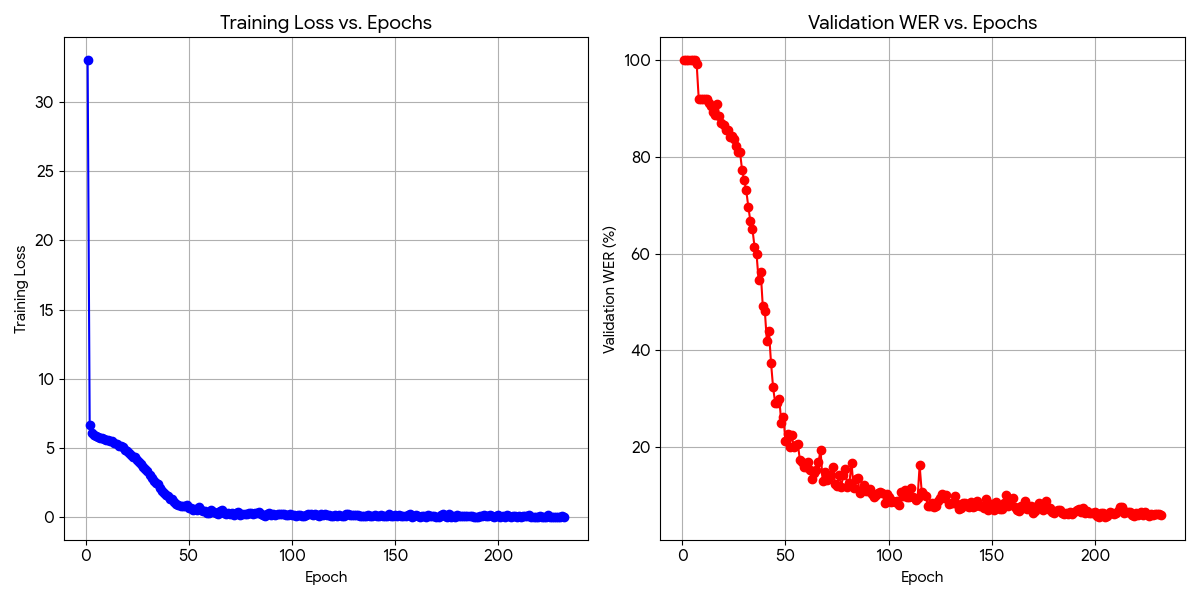
\includegraphics[width=1\linewidth]{WER Loss.png}
    \caption{A plot showing the CTC loss and WER for both the training and development sets over 225 epochs. Both curves show a steady decrease, indicating that the model is learning effectively and generalizing well to the unseen development data}
    \label{fig:training_progress}
\end{figure}

\subsection{Error Analysis}
Error analysis of test predictions highlighted model limitations and failure modes. A test WER of 12.70\% resulted from 1,474 errors over 18,017 words, with 607 substitutions, 583 deletions, and 284 insertions. Error patterns in Table~\ref{tab:gloss_comparison} show deletions of repeated signs, insertions of plausible yet incorrect glosses, and substitutions among similar signs. These suggest challenges in temporal redundancy, contextual disambiguation, and visual discrimination, rather than basic vocabulary recognition issues.

\begin{table}[h]
    \centering
    \begin{tabularx}{\columnwidth}{c >{\Centering}X >{\Centering}X}
        \toprule
        \textbf{ID} & \textbf{Ground Truth Gloss} & \textbf{Predicted Gloss} \\
        \midrule
        2  & \textarabic{معرفه معلم لغه اشاره} & \textarabic{معرفه لغه اشاره} \\
        19 & \textarabic{انا اخ كتابه} & \textarabic{انا كتابه} \\
        21 & \textarabic{انا واحد مشاهده جميل} & \textarabic{انا ماضي مشاهده قرد جميل} \\
        38 & \textarabic{قط صغير تحت طاوله} & \textarabic{قط صغير تحت} \\
        46 & \textarabic{سوال هو سوال} & \textarabic{سوال هو} \\
        \bottomrule
    \end{tabularx}
    \caption{Comparison of Ground Truth Gloss and Predicted Gloss}
    \label{tab:gloss_comparison}
\end{table}

\begin{table*}[t] % Use [t] for top of page
    \centering
    \begin{tabular}{lcc}
        \toprule
        \textbf{Architecture Experiment} & \textbf{Dev WER (\%)} & \textbf{Test WER (\%)}  \\
        \midrule
        Stochastic Weight Averaging (SWA) & 11.26& 18.53\\
        Wider Beam (Beam Width = 20) & 11.66 & 20.67  \\
        Macaron-Net-inspired (Baseline) & 7.86 & 16.33  \\
        Deep Conformer& 7.93 & 14.75  \\
        Squeeze-and-Excite Conformer & 22.31 & 98.88  \\
        Data-Centric CSLRConformer& 5.60 & 12.70  \\
        \bottomrule
    \end{tabular}
    \caption{Comparison of Word Error Rate (WER) for Different Architecture Experiments}
    \label{tab:arch_comparison_wide}
\end{table*}

\subsection{Ablation Study: Impact of Feature Selection}
To rigorously evaluate the contribution of the EDA-driven feature selection strategy, a comprehensive ablation study was conducted. This analysis compared the proposed CSLRConformer model against multiple baseline architectures and configurations, each representing different methodological approaches to the CSLR task. 

\textbf{Feature Selection Impact:} For all alternative architectures in this comparison, the complete set of 86 keypoints was utilized, whereas the proposed CSLRConformer leverages only 82 keypoints selected through the EDA-driven feature selection process. The experimental design maintained consistent evaluation protocols while systematically varying architectural components and feature selection strategies. The comparative analysis, presented in Table~\ref{tab:arch_comparison_wide}, reveals substantial performance differentials across different approaches within the internal experimental framework.

The baseline configurations, including Stochastic Weight Averaging (SWA) implementation, wider beam search strategies (beam width = 20), and alternative Conformer architectures such as Deep Conformer and Squeeze-and-Excite variants, consistently underperformed relative to the proposed data-centric approach. Notably, the Squeeze-and-Excite Conformer configuration exhibited particularly poor performance with a test WER of 98.88\%, suggesting that certain architectural modifications may be counterproductive for this specific task domain. 

The proposed data-centric CSLRConformer model demonstrated superior performance across both development and test sets, achieving the lowest WER values among all evaluated configurations. Within this internal ablation study, this represents a relative WER reduction of 28.8\% on the development set and 22.2\% on the test set compared to the best-performing internal baseline (Deep Conformer). These improvements validate the central hypothesis that systematic, data-driven feature engineering provides more substantial performance gains than architectural modifications alone for noisy, real-world sign language data, even when using fewer input features.

%-------------------------------------------------------------------------
\subsection{Analysis of Results}

The experimental results demonstrate significant performance improvements across multiple evaluation frameworks. Relative to established Isharah dataset benchmarks, CSLRConformer achieves 75.1\% and 53.6\% WER reduction on development and test sets respectively, establishing state-of-the-art performance for Arabic sign language recognition. Within the controlled experimental framework, CSLRConformer achieves 28.8\% and 22.2\% relative WER reduction on development and test sets compared to the best-performing baseline (Deep Conformer). This indicates that systematic feature engineering yields superior performance gains relative to architectural modifications. Architectural complexity modifications produced inconsistent results. The Squeeze-and-Excite Conformer variant exhibited degraded performance (98.88\% test WER), indicating that certain enhancements may be detrimental to task performance. Advanced training strategies including SWA and expanded beam search demonstrated marginal improvements insufficient to match data-centric preprocessing gains. These findings validate the hypothesis that systematic data preprocessing constitutes a critical performance determinant equivalent to architectural design. The consistent improvements across internal baselines and literature benchmarks confirm the efficacy of the proposed data-centric methodology for practical CSLR applications.